\section{Derivation of $C_{l}$ rolling moment coefficient}
In this part of the project the rolling moment coefficient of the J35 Draken is to be calculated.
For the simulation, the model of fig.\ref{fig:model} was used:

\begin{figure}[H]
    \begin{center}
        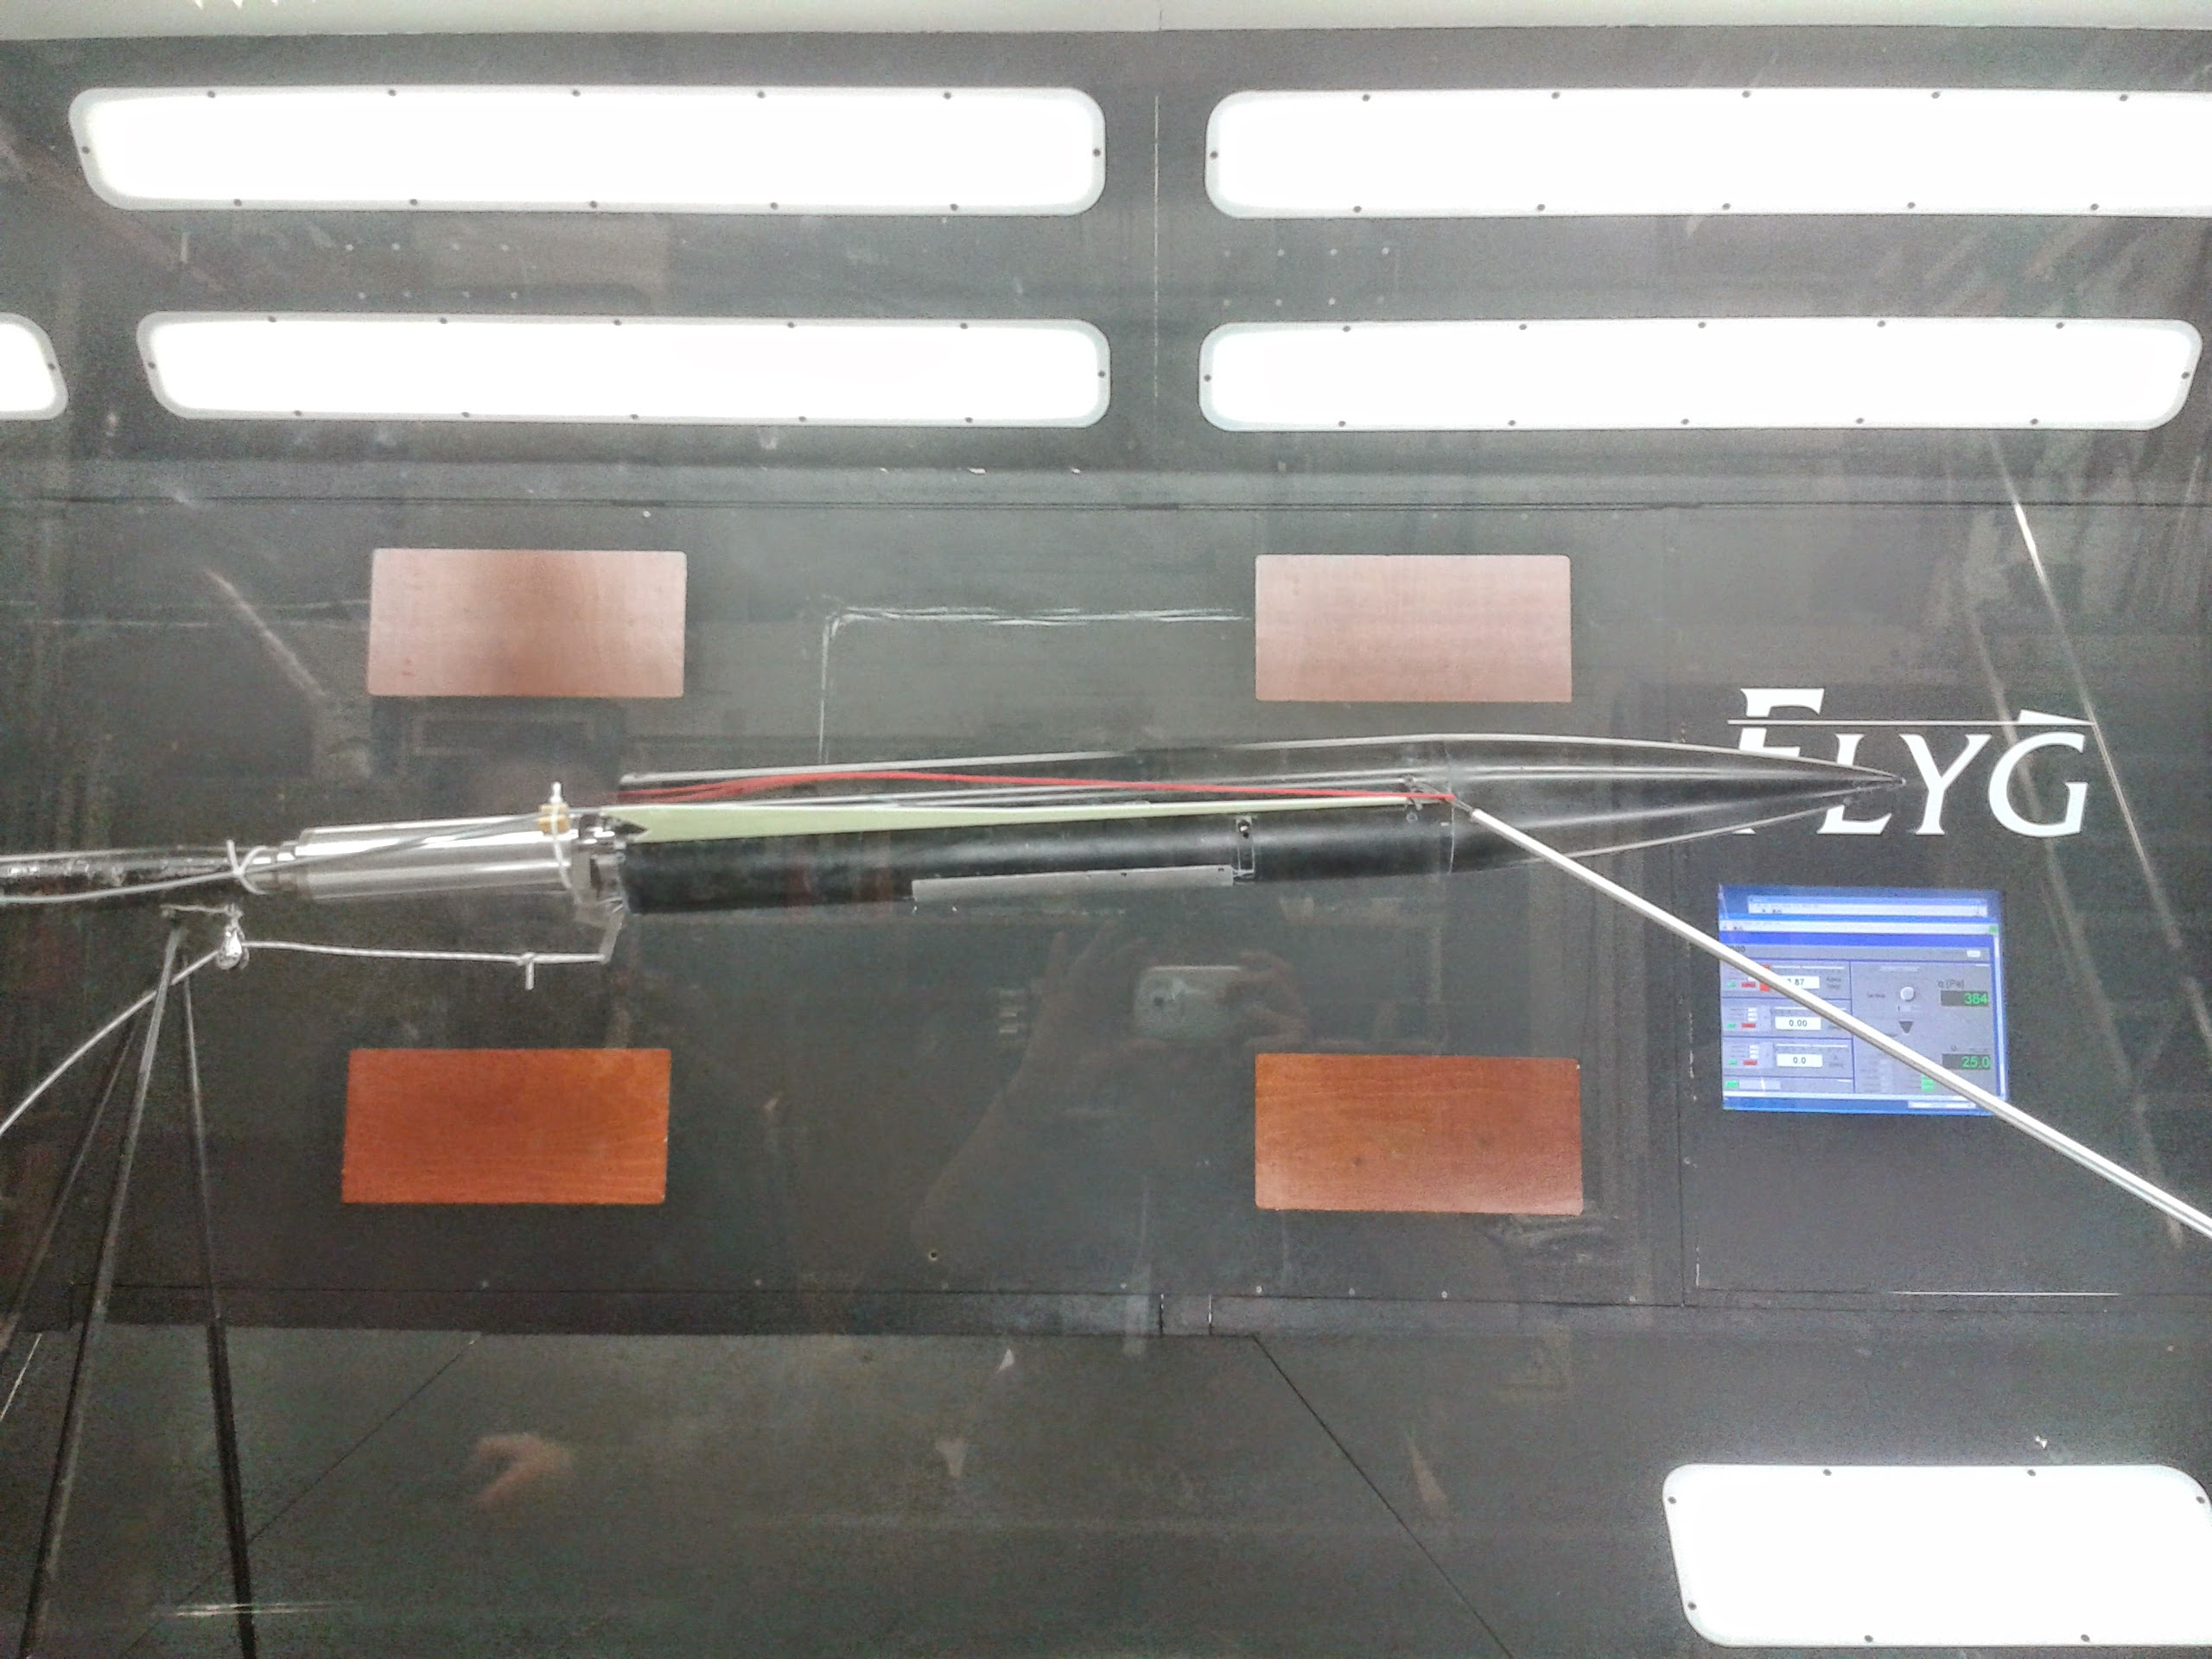
\includegraphics[width = 0.6\textwidth]{model.jpg} % Just THIS!!!
    \end{center}
    \caption{Picture of model during wind tunnel test}
    \label{fig:model}
\end{figure}

\subsection{Simulation Considerations}

The following can be stated when comparing the J35 Draken aircraft with the wind tunnel model used(fig.~\ref{fig:model})
\begin{itemize*}
    \item Apparently the major difference is the \textit{absence of the fin}. 
        This fact eventually caused considerable divergence between the values computed during the 
        simulation and the data extracted from Draken data diagramms provided.
    \item The wind tunnel model scale was 1:14.7 except for the bodywidth
        and noselength. 
\end{itemize*}


\subsection{Mathematical Modelling}
To proceed with the analysis and the computation of $C_{lp}, C_{l\beta}$ parameters, 
a valid mathematical model needs to be derived first. 
If We implement the Newton's second law for the rolling movement
we can derive equation \ref{eqn:newton_angular}.

\begin{equation}
    \Sigma T = I_{xx}\ddot{\phi} \Rightarrow 
    l - C\dot{\phi} - k\phi = I_{xx}\ddot{\phi},
    \label{eqn:newton_angular}
\end{equation}

\nomenclature{$I_{xx}$}{Rolling moment of inertia}%
\nomenclature{$C$}{Damping coefficient of aircraft rolling motion}%
\nomenclature{$q$}{Dynamical Pressure}%
\nomenclature{$C$}{Damping coefficient of aircraft rolling motion}%
\nomenclature{$k$}{Spring coefficient of aircraft rolling motion}%
\nomenclature{$p$}{Roll angle derivative}%
\nomenclature{$\rho$}{Density of air}%
\nomenclature{$u$}{Projection of velocity on the x-axis of airplane (Body-fixed system)}%
\nomenclature{$v$}{Projection of velocity on the y-axis of airplane (Body-fixed system)}%
\nomenclature{$w$}{Projection of velocity on the w-axis of airplane (Body-fixed system)}%

\noindent where $C\dot{\phi}$ is the moment exerted due to the (mechanical) damping and $k\phi$ is
the moment due to the (mechanical) spring stiffness of the device holding the airplane during the simulation.
For the calculation of the rolling moment the following equations can be used:
\begin{eqnarray}
    l &=& C_l q b S \label{eqn:roll_moment} \label{eqn:l}\\
    C_l &=&  C_{lp}\frac{pb}{2u} + C_{l\beta}\beta \label{eqn:cl}\\
    p &=&\dot{\phi} \\
    q &=&  \frac{1}{2}\rho u^2 
\end{eqnarray}

\nomenclature{$l$}{Rolling moment}%
\nomenclature{$C_l$}{Rolling moment coefficient}%

A sufficient model of calculating $C_l$ - the rolling moment coefficient - is given in equation
\ref{eqn:cl}. According to this, $C_l$ is a function of $C_{lp}$ the \textit{damping-in-roll}
coefficient and $C_{l\beta}$ the dihedral effect.
$C_{lp}$ expresses the resistance of the airplane to rolling 
\cite{etkin_dynamics_1972}, while $C_{l\beta}$ expresses the change in rolling moment 
coefficient per degree of change in the sideslip angle $\beta$. A sufficient relation to 
calculating $\beta$ can be the following:
\begin{equation}
    \beta = \alpha \phi
    \label{eqn:beta}
\end{equation}

\nomenclature{$\beta$}{Sideslip angle}%

\noindent If we now substitute the expression of rolling moment \ref{eqn:l} into the initial equation
\ref{eqn:newton_angular}, and move all the $\phi, \dot{\phi}$ terms to the other side of the equation
we can end up with the following second order differential equation:

\begin{equation}
    I_{xx}\ddot{\phi} + \dot{\phi}\big(C_{mech} - \frac{C_{lp}Sb^2q}{2u}\big) + \big(k - C_{l\beta}aqbS\big)\phi = 0
    \label{eqn:ode_used}
\end{equation}

\noindent The analytical solution of \ref{eqn:ode_used} for the general case of complex roots
(which is what we expect due to the oscillatory behavior of the model movement) is the following:

\begin{eqnarray}
    \phi &=&  c_1e^{\alpha' x}cos(\beta' x) + c_2e^{\alpha' x} sin(\beta' x) \label{eqn:phianal}\\
    \alpha' &=&  -\frac{\beta}{2\alpha} \notag\\
    \beta' &=&  \frac{\sqrt{4ac - b^2}}{2a} \notag\\
\end{eqnarray}

where $\alpha, \beta, c$ are the coefficients of \ref{eqn:ode_used} respectively:
\begin{eqnarray}
    \alpha &=& I_{xx} \label{eqn:alpha}\\
    \beta &=&  C_{mech} - \frac{C_{lp}Sb^2q}{2u} \label{eqn:beta}\\
    c &=&  k - C_{l\beta}aqbS \label{eqn:c}
\end{eqnarray}

\nomenclature{$b$}{Airplane Span}%
\nomenclature{$S$}{Airplane Surface Area}%
\nomenclature{$C_{lp}$}{Damping in Roll Coefficient}%
\nomenclature{$C_{l\beta}$}{Dihedral Effect}%

\noindent To get the analytical solution of the roll rate $\dot{\phi}$ we take the derivative 
of \ref{eqn:phianal}:

\begin{eqnarray}
    \dot{\phi} &=&   \big(-C_1 \beta' sin(\beta' x) + C_2 \beta' cos(\beta' x) \big) e^{\alpha' x} =\notag\\
     &=&  \beta'\big(-C_1+C_2\big)e^{\alpha'}x\big(sin(\beta'x) + cos(\beta'x)\big) = \notag\\
     &\Rightarrow& \big\{A = \beta' \big(-C_1+C_2\big) \quad \big\} \Rightarrow \notag\\
     \dot{\phi} &=& Ae^{\alpha'x}\big(sin(\beta'x) + cos(\beta'x)\big) \label{eqn:panal} = \notag\\
     &\Rightarrow&  \big\{asin(\theta) + bcos(\theta) = Rsin\big(\theta \pm \alpha\big)\big\}\Rightarrow \notag\\
     \dot{\phi} &=& Ae^{\alpha'x}\big(sin(\beta'x + \Theta \big) \label{eqn:panal} \label{eqn:panal}
\end{eqnarray}

\subsection{Derivation of \textit{damping-in-roll} derivative $C_{lp}$}

To derive the $C_{lp}$ parameter, we first need to extract information out of 
the experimental data gathered. The oscillation of the rolling motion can be modelled as a 
decaying sinusoidal function of time. Therefore we can fit a function 
of the form~\ref{eqn:panal} in the data and estimate each parameter 
by using the least squares method.

The data fit procedure uses the Fourier transform to extract the basic frequency as well as the least squares method.
Figures~\ref{fig:datafit1},\ref{fig:datafit2} show some examples of the data fits that demonstrate the efficiency of the 
approximation algorithm used.

\begin{figure}[H]
        \centering
        \begin{subfigure}[b]{0.48\textwidth}
                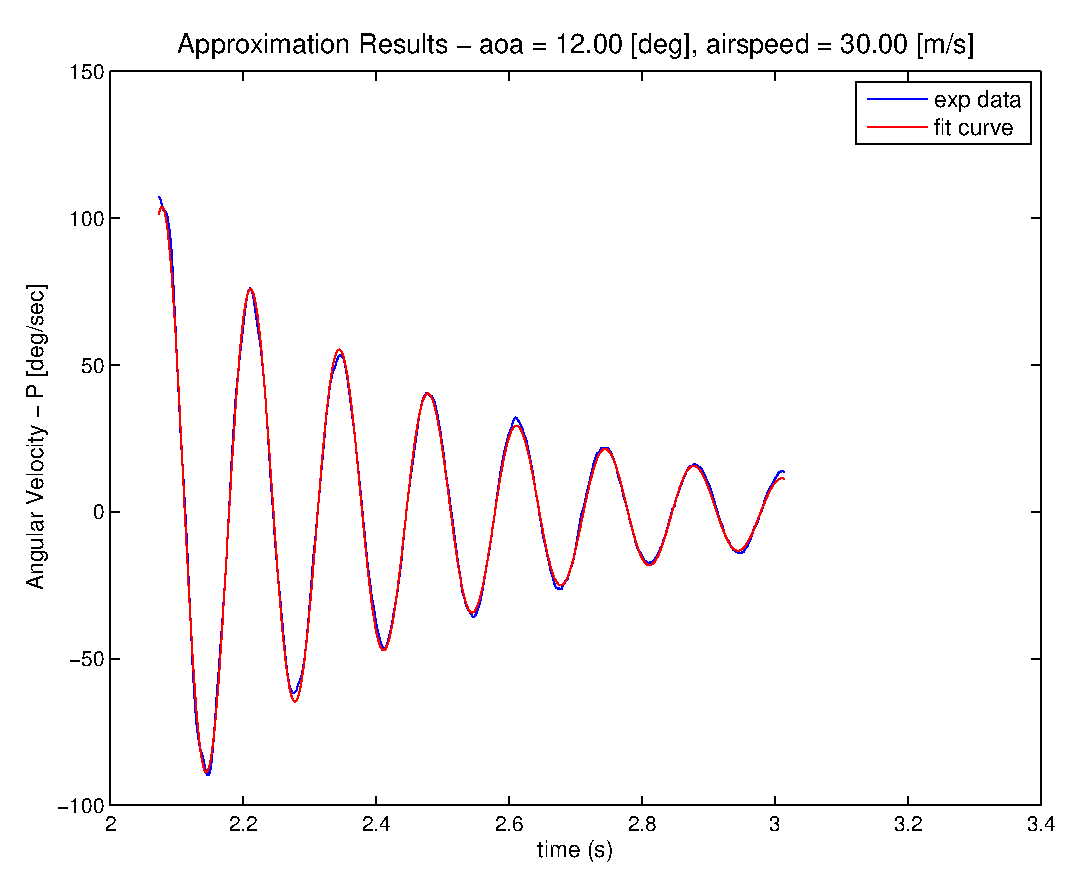
\includegraphics[width=\textwidth]{datafit_clp1}
                \caption{V = 35 $\sfrac{m}{s}$}
                \label{fig:datafit1}
        \end{subfigure}%
        ~
        \begin{subfigure}[b]{0.48\textwidth}
                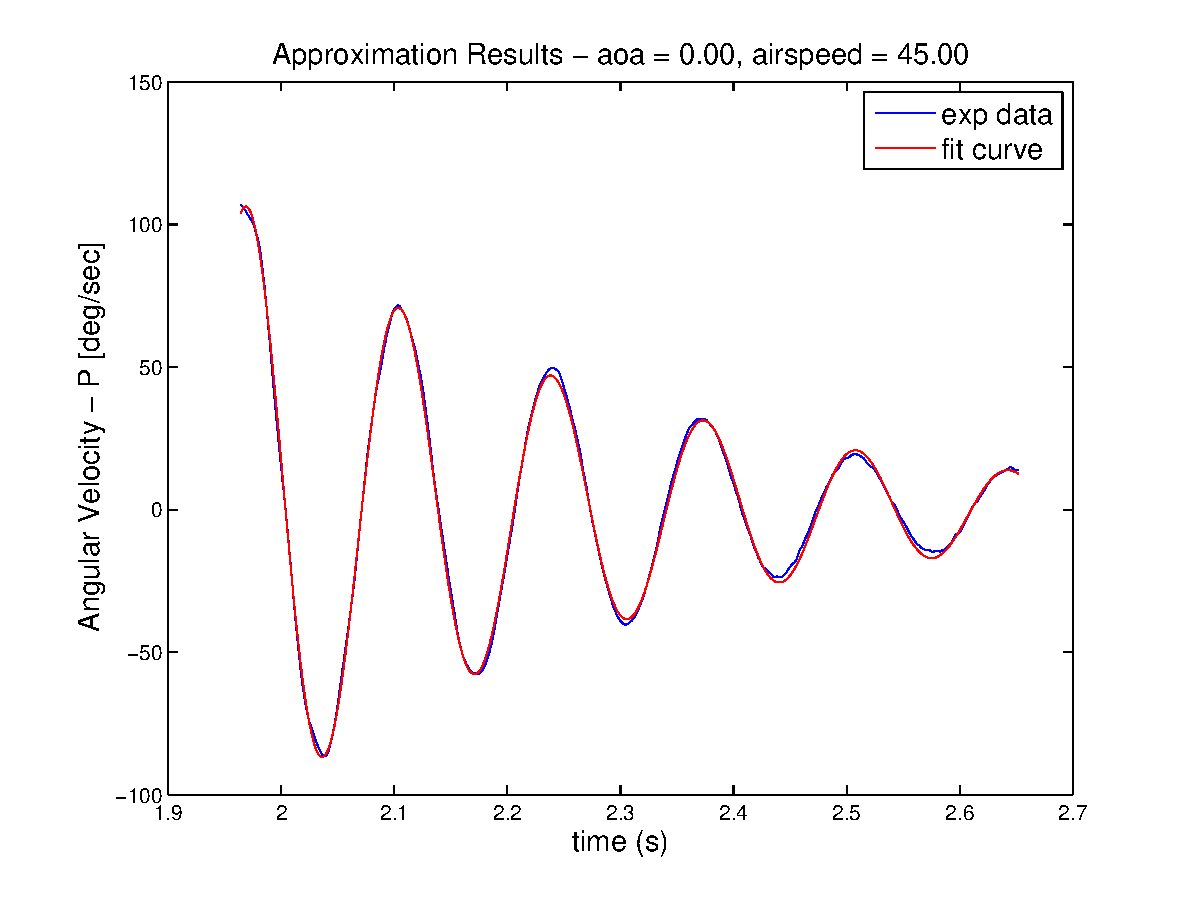
\includegraphics[width=\textwidth]{datafit_clp2}
                \caption{V = 45 $\sfrac{m}{s}$}
                \label{fig:datafit2}
        \end{subfigure}

        \caption{Examples of the data fitting procedure}
\end{figure}

To derive only the value of the $C_{lp}$ parameter we have to take into account \textit{only the data for $\alpha = 0$},
because otherwise $C_{l\beta}$ starts to play a role in the behavior of the oscilation (see eq.~\ref{eqn:ode_used}).

To extract the maximum amount of data and be as accurate as possible we \textit{process all the $\alpha = 0$ measurements taken during the laboratory sessions.}
\footnote{The reader is encouraged to refer to stiff.m of the code part for the actual implementation}.

The procedure can be summarised in the next steps:
\begin{enumerate}
    \item Calculation of $C_{mech}, I_{xx}$\footnote{I know that $I_{xx} = \sqrt{\frac{k}{\omega^2}}$ where k
    has already been determined experimentally.} using one of the  $\alpha = 0,\, V = 0$ measurements available.
    \item Approximation of the n-v \footnote{n is the damping coefficient, equivalent to $\beta'$ of eq.~\ref{eqn:panal}}curve by using a wide rage of velocities to calculate n-values and by using the least squares method.
    \item Calculation of the n-v  curve slope from which knowing every other quantity I can extract an estimation of the $C_{lp}$ value.
\end{enumerate}

Using this strategy we can now derive the approximation curve of the n-v points
presented in fig~\ref{fig:v_n_graph}. Using this graph and the methodology described 
in the previous steps we can now conclude to the value of $C_{lp}$:

\begin{equation}
    C_{lp} \simeq -0.190
\end{equation}
Since this value is (strictly) negative and is 
close to the data given for the real aircraft~\cite{database}(for $\alpha = 0$), 
We can conclude that it is a logical estimation of the damping-in-roll coefficient.

\begin{figure}[th]
    \begin{center}
        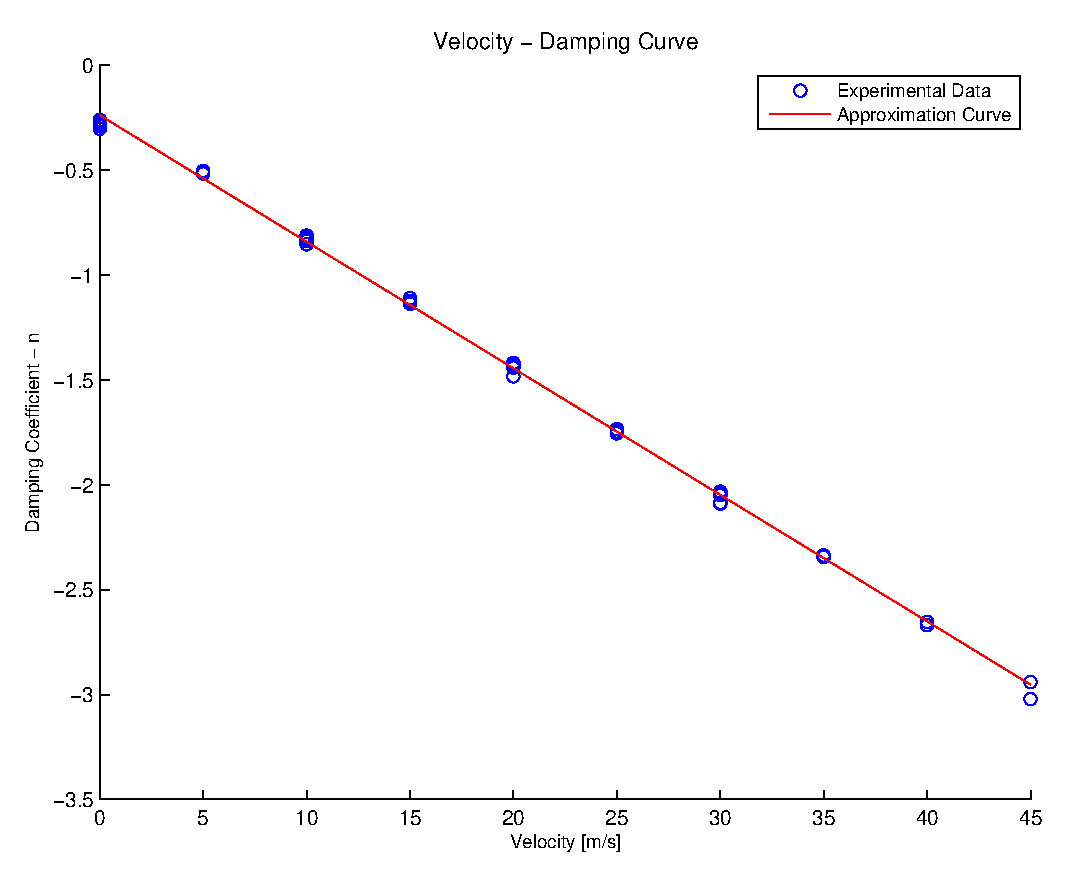
\includegraphics[width=0.7\textwidth]{v_n_graph} % Just THIS!!!
    \end{center}
    \caption{Velocity - damping approximation curve}
    \label{fig:v_n_graph}
\end{figure}



\subsection{Derivation of the \textit{Dihedral effect} $C_{l\beta}$}

We use the same strategy as in the derivation of $C_{lp}$ to find a formula for 
calculating $C_{l\beta}$. $C_{l\beta}$ appers only in the formula of $\beta'$ (see eq. ~\ref{eqn:phianal})
which corresponds to the natural frequency of the aircraft oscillation. Executing the 
necessary computations, we can find an expression for the calculation of $C_{l\beta}$.

\begin{align}
    \omega_n &= \beta' = \frac{\sqrt{4\alpha c - \beta^2}}{2\alpha} \Rightarrow \notag\\
    \omega_n^2 &= \frac{4\alpha c - \beta^2}{4\alpha^2} \Rightarrow \notag\\
    &\Rightarrow \{\textrm{Substituting quantities from eq.~\ref{eqn:alpha}-\ref{eqn:c}} \}\Rightarrow \notag\\
    \omega_n^2 &= -\bigg(\frac{C_{l\beta}\alpha \rho bS}{2I_{xx}} + \frac{C_{lp}^2\rho S^2 b^4 \rho^2}{64I_{xx}^2}\bigg)V^2
    + \bigg(\frac{C_{mech}C_{lp}Sb^2\rho}{8I_{xx}^2}\bigg)V
    + \big(4I_{xx}k - C_{mech}^2\big) \label{eqn:wn2_V}
\end{align}

If we now fit the experimental data (V, $\omega_n^2$) into a quadratic polynomial model of the form 
$ax^2 + bx + c$ using the least squares method and extract the 
coefficients a, b, c we can find an analytical formula for $C_{l\beta}$.
So taking this into account and knowing that $C_{l\beta}$ appears in the expression
of the first coefficient of the $V-\omega_n^2$ curve, we end up with the following expresion:

\begin{equation}
    C_{l\beta} = -\bigg(\frac{2I_{xx}\times coeff(1)}{\alpha \rho bS} + 
    \frac{C_{lp}^2Sb^3I_{xx}}{32I_{xx}^2\alpha b}\bigg)
    \label{eqn:clb_calc}
\end{equation}

As we can see from eq~\ref{eqn:clb_calc} $C_{l\beta}$ is a function of the 
first coefficient of the fitting curve (coeff(1)), of $C_{lp}$ which was previously
calculated, and of $\alpha$. To proceed to the actual calculation, 
we fit quadratic polynomial curves over the $V-\omega^2$ pairs for each value of $\alpha$
and therefore caclulate the $C_{l\beta}$ values.
\footnote{We consider only the values of $\alpha$ for which sufficient experimental data has been gathered.
See stiff.m for the actual implementation}

Having executed the above procedure we end up with the following graphs 
for different $\alpha$ angles:
\footnote{Some basic filtering was needed for the gathered experimental points. 
More specifically points that were outside the range of 3$sigma$ where $\sigma$
is the standard deviation of the distribution were ruled out.}

\begin{figure}[H]
    \begin{center}
        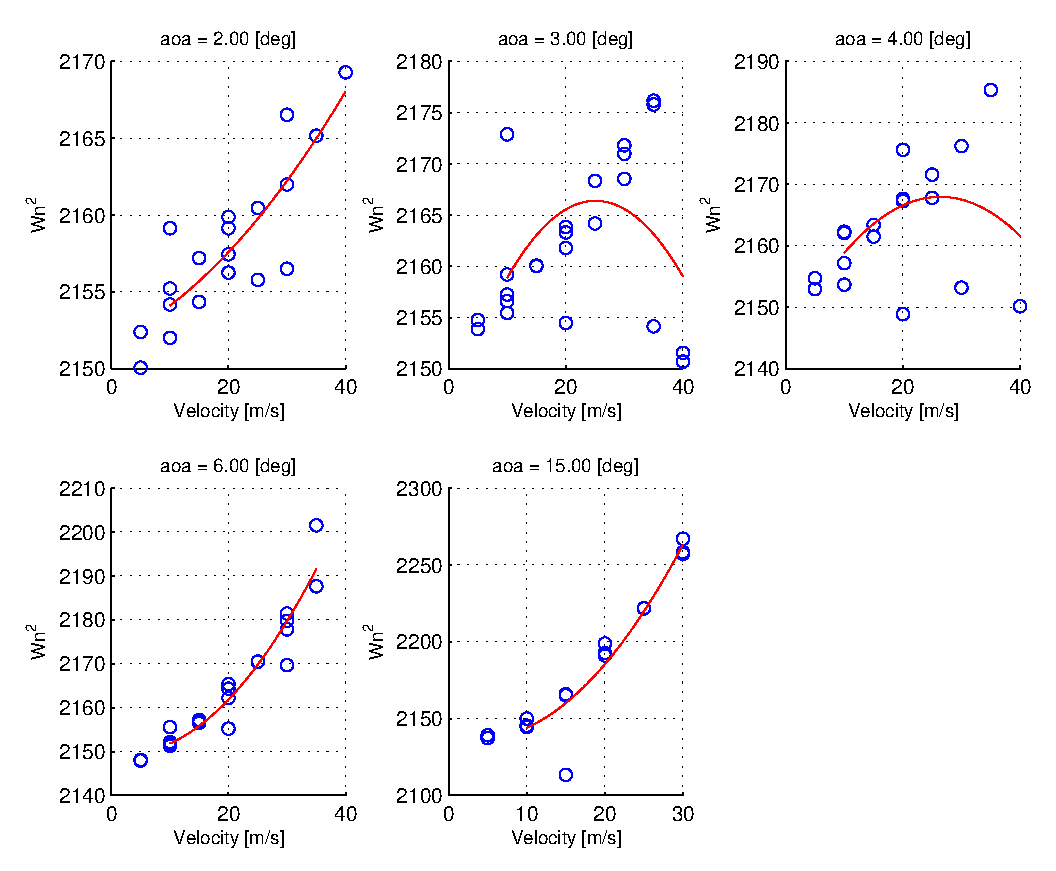
\includegraphics[width = 0.8\textwidth]{v_wmega2_graph} % Just THIS!!!
    \end{center}
    \caption{Fitting of polynomial curve into experimental data, for different $\alpha$ values}
    \label{fig:v_wmega2_graph}
\end{figure}

If we now extract $C_{l\beta}$ using eq.~\ref{eqn:clb_calc} we end up with the 
following values:

\begin{itemize}
    \item $\alpha = 2\degree\; \rightarrow \beta  = -0.0026$
    \item $\alpha = 3\degree\; \rightarrow \beta  = 0.0048$
    \item $\alpha = 4\degree\; \rightarrow \beta  = 0.0037$
    \item $\alpha = 6\degree\; \rightarrow \beta  = -0.0037$
    \item $\alpha = 15\degree\; \rightarrow \beta  = -0.0063$
\end{itemize}

